% Options for packages loaded elsewhere
\PassOptionsToPackage{unicode}{hyperref}
\PassOptionsToPackage{hyphens}{url}
\documentclass[
  11pt,
]{article}
\usepackage{xcolor}
\usepackage[margin=2.5cm]{geometry}
\usepackage{amsmath,amssymb}
\setcounter{secnumdepth}{5}
\usepackage{iftex}
\ifPDFTeX
  \usepackage[T1]{fontenc}
  \usepackage[utf8]{inputenc}
  \usepackage{textcomp} % provide euro and other symbols
\else % if luatex or xetex
  \usepackage{unicode-math} % this also loads fontspec
  \defaultfontfeatures{Scale=MatchLowercase}
  \defaultfontfeatures[\rmfamily]{Ligatures=TeX,Scale=1}
\fi
\usepackage{lmodern}
\ifPDFTeX\else
  % xetex/luatex font selection
\fi
% Use upquote if available, for straight quotes in verbatim environments
\IfFileExists{upquote.sty}{\usepackage{upquote}}{}
\IfFileExists{microtype.sty}{% use microtype if available
  \usepackage[]{microtype}
  \UseMicrotypeSet[protrusion]{basicmath} % disable protrusion for tt fonts
}{}
\makeatletter
\@ifundefined{KOMAClassName}{% if non-KOMA class
  \IfFileExists{parskip.sty}{%
    \usepackage{parskip}
  }{% else
    \setlength{\parindent}{0pt}
    \setlength{\parskip}{6pt plus 2pt minus 1pt}}
}{% if KOMA class
  \KOMAoptions{parskip=half}}
\makeatother
\usepackage{longtable,booktabs,array}
\usepackage{calc} % for calculating minipage widths
% Correct order of tables after \paragraph or \subparagraph
\usepackage{etoolbox}
\makeatletter
\patchcmd\longtable{\par}{\if@noskipsec\mbox{}\fi\par}{}{}
\makeatother
% Allow footnotes in longtable head/foot
\IfFileExists{footnotehyper.sty}{\usepackage{footnotehyper}}{\usepackage{footnote}}
\makesavenoteenv{longtable}
\usepackage{graphicx}
\makeatletter
\newsavebox\pandoc@box
\newcommand*\pandocbounded[1]{% scales image to fit in text height/width
  \sbox\pandoc@box{#1}%
  \Gscale@div\@tempa{\textheight}{\dimexpr\ht\pandoc@box+\dp\pandoc@box\relax}%
  \Gscale@div\@tempb{\linewidth}{\wd\pandoc@box}%
  \ifdim\@tempb\p@<\@tempa\p@\let\@tempa\@tempb\fi% select the smaller of both
  \ifdim\@tempa\p@<\p@\scalebox{\@tempa}{\usebox\pandoc@box}%
  \else\usebox{\pandoc@box}%
  \fi%
}
% Set default figure placement to htbp
\def\fps@figure{htbp}
\makeatother
\setlength{\emergencystretch}{3em} % prevent overfull lines
\providecommand{\tightlist}{%
  \setlength{\itemsep}{0pt}\setlength{\parskip}{0pt}}
\usepackage{bookmark}
\IfFileExists{xurl.sty}{\usepackage{xurl}}{} % add URL line breaks if available
\urlstyle{same}
\hypersetup{
  pdftitle={IMDb Ratings vs.~Votes},
  pdfauthor={Eveline Verhage, Eefje van der Sanden, Sanne van der Wiel, Jeroen Swolfs, Edwin van Zon},
  hidelinks,
  pdfcreator={LaTeX via pandoc}}

\title{IMDb Ratings vs.~Votes}
\author{Eveline Verhage, Eefje van der Sanden, Sanne van der Wiel,
Jeroen Swolfs, Edwin van Zon}
\date{2025-10-08}

\begin{document}
\maketitle

{
\setcounter{tocdepth}{2}
\tableofcontents
}
\#1. Introduction

The Internet Movie Database (IMDb) is one of the most widely used online
platforms for film and television information, containing millions of
titles along with user-generated ratings and vote counts. It serves as a
valuable resource for studying audience preferences and perceptions of
quality across a diverse range of genres and formats.

This study investigates the relationship between popularity (measured by
the number of votes) and perceived quality (average IMDb rating) of
films and series. Using IMDb data, the analysis examines whether highly
rated titles also attract more votes, or whether popularity and quality
diverge. Furthermore, it explores whether this relationship differs
across genres and between movies and series (i.e., content form).

\#2. Theoretical Framework and Research Motivation The relationship
between the number of votes and the average rating of movies provides
valuable insights into audience behaviour and preferences. Understanding
this relationship can inform film studios, reviewers, and marketing
professionals about how viewers engage with content and express their
opinions online.

Based on prior research on the polarization effect - the tendency for
individuals with strong positive or negative opinions to be more likely
to share them - this study expects the relationship between the number
of votes and average rating to be non-linear (quadratic) rather than
linear. Two competing hypotheses are proposed regarding the shape of
this relationship. First, both highly rated and poorly rated titles may
attract more attention and engagement, as individuals with strong
opinions are more likely to share them. This would produce a concave
upward (U-shaped) relationship between rating and vote count.
Conversely, widely viewed mainstream films might receive a high number
of ratings that are relatively moderate, reflecting a broader audience
appeal. This would result in a concave downward (inverted U-shaped)
relationship.

Moreover, the relationship between ratings and number of votes Genres
may attract distinct audience segments that vary in their rating
behavior---mainstream genres might yield different rating distributions
compared to niche ones. Likewise, differences between movies and series,
such as viewing length and audience engagement patterns, could also
influence the relationship between popularity and perceived quality. As
such the analysis also controls for (1) differences in genre and (2)
differences between movies and series.

\#3. Research Question The current project sets out to answer the
following research question: \emph{What is the relationship between the
number of votes and the average rating of movies on IMDb?}

Additionally, this relationship may depend on several sub-factors,
resulting in two sub-questions: 1.Does the relationship between number
of votes and average rating differ across movie genres (escapist
(fantasy, comedy, romance) and heavy (drama, thriller))? 2.Does the
relationship between number of votes and average rating differ across
movies and series (i.e.~content form)?

\#4. Data \#\#4.1. Data Sourcing We programmatically downloaded two
public IMDb datasets: • title.basics (title type, year, genres) •
title.ratings (average rating, number of votes)

Given the substantial size of the files and the need for a manageable
data set for our analysis, we have selected a reduced sample of 200,000
observations from the IMDb data set. This sample size enables us to
conduct thorough statistical analyses while ensuring efficiency. A seed
was set at 123 to ensure that analysis is run with the same data.

\#\#4.2. Data preparation To ensure that the IMDb datasets were
consistent and suitable for statistical analysis, the two source files
(title.basics and title.ratings) were merged using the unique identifier
tconst using inner-join. An inner join was chosen because it retains
only titles that appear in both datasets (i.e., titles that have both
descriptive information and user ratings).This approach ensures that
every observation in the final dataset contains complete and relevant
information for the analysis.

Data cleaning steps included: • Casting startYear to integer -- Ensured
that the year variable could be used for temporal filtering, grouping,
and period classification. • Filtering only movies and series --
Excluded other types of titles (e.g., short films, video games, or
documentaries) to maintain a consistent comparison across similar
content forms. • De-duplicating titles -- Removed potential duplicates
in the IMDb data to avoid over-representation of the same title. •
Dropping titles with fewer than 20 votes -- After data inspection, we
found that many titles had just a few votes (ie data is right skewed).
Titles with very few votes were considered unreliable indicators of
audience opinion; removing them reduced statistical noise whilst
retaining enough variation to answer the primary research question. •
Mapping genres into three broader families (Escapist, Heavy, Mixed) --
Simplified the complex and overlapping IMDb genre system into
analytically meaningful categories, improving interpretability across
genres. The Mixed genre was filtered out; this would overcomplicate
analysis (three levels of an independent variable with multiple levels
of moderators) and deletion also resulted in a more clean measure of the
moderating effect of genres.

Additional features were engineered to support the analysis: • votes2 --
The squared number of votes, used to capture potential non-linear
relationships between popularity and quality. • log\_votes and
log\_votes2 -- Logarithmic transformations of vote count and its square
to reduce skewness and handle large disparities between extremely
popular and niche titles. • period -- Classified titles into four
historical periods (Pre-War, Interwar, Post-War, Modern), allowing
temporal trends in popularity and rating behavior to be explored. •
rating\_category -- Grouped IMDb ratings into ordinal categories (Very
Bad to Excellent), providing a more intuitive interpretation of
perceived quality.

These steps produced three progressively refined datasets used
throughout the analysis: • imdb\_clean -- The base cleaned dataset after
initial filtering and deduplication. • imdb\_enriched -- The dataset
with added genre family and period variables. • imdb\_analysis -- The
final, analysis-ready dataset including transformations and derived
metrics for modeling and

\#\#4.3. Variables Stuk Sanne van de Readme (ie tabellen)

\#5. Research Method \#\#5.1. Main Analysis To empirically test the
research question, a series of linear regression models were estimated
using IMDb data. In these models, the dependent variable (DV) is the
average IMDb rating, representing viewers' perceived quality of a title.
The independent variable (IV) is the number of votes, log-transformed to
correct for skewness in the distribution of popularity across titles.
Given theoretical expectations from the polarization effect, a squared
term of the log number of votes (log\_votes²) was added to capture
potential non-linear (quadratic) patterns between popularity and
perceived quality. The period of release was included as a control
variable to account for differences in rating behavior over time. To
address the sub-questions, moderator analyses were performed by adding
interaction terms between the vote variables and (1) genre family and
(2) content type (movie vs.~series).These moderators allow us to test
whether the relationship between popularity and quality depends on genre
characteristics or format differences.

As such, we performed a moderated regression analysis, broken up into
several pieces to answer our research (sub)question(s). Linear
regression was chosen as the primary analytical technique because it
allows for straightforward interpretation of main and interaction
effects and flexible testing of both linear and non-linear
relationships.

\#\#5.2. Regressions Four linear regression models were estimated
sequentially to address the research question and sub-questions.

\textbf{Model 1: Baseline linear model} ``averageRating''=β\_0+β\_1
(log⁡\_votes)+β\_2 (``period'')+ϵ

This model assesses the linear relationship between the log-transformed
number of votes and the average rating, controlling for time period.

\textbf{Model 2: Quadratic model} ``averageRating''=β\_0+β\_1
(log⁡\_votes)+β\_2 (log⁡\_votes\^{}2)+β\_3 (``period'')+ϵ

This model tests for a non-linear (quadratic) relationship between
rating and number of votes; allowing to answer the main research
question. An ANOVA comparison between Model 1 and Model 2 determines
whether the quadratic term significantly improves model fit.

\textbf{Model 3: Genre as a moderator} ``averageRating''=β\_0+β\_1
(log⁡\_votes)+β\_2 (log⁡\_votes\^{}2)+β\_3 (``genre\_family'')+β\_4
(log⁡\_votes×``genre\_family'')+β\_5
(log⁡\_votes\^{}2×``genre\_family'')+ϵ

This model investigates whether the votes--ratings relationship differs
between Escapist and Heavy genres.

\textbf{Model 4: Content form as a moderator}
``averageRating''=β\_0+β\_1 (log⁡\_votes)+β\_2 (log⁡\_votes\^{}2)+β\_3
(``type'')+β\_4 (log⁡\_votes×``type'')+β\_5 (log⁡\_votes\^{}2×``type'')+ϵ

This model tests whether the relationship varies between movies and
series, given their differences in audience engagement and viewing
context.

Note that additionally, we planned to run a fifth model with rating as a
category variable. However, when running this model we realized that
meaningful categories were hard to define based on ratings (is a rating
of 1.9 significantly worse than 2.0 if categories are defined as 1-2,
3-4, 5-6 etc). As such, this analysis was not included in the main
reporting.

The table below summarizes the regressions.

\begin{longtable}[]{@{}
  >{\raggedright\arraybackslash}p{(\linewidth - 6\tabcolsep) * \real{0.2800}}
  >{\raggedright\arraybackslash}p{(\linewidth - 6\tabcolsep) * \real{0.1600}}
  >{\raggedright\arraybackslash}p{(\linewidth - 6\tabcolsep) * \real{0.2000}}
  >{\raggedright\arraybackslash}p{(\linewidth - 6\tabcolsep) * \real{0.3600}}@{}}
\toprule\noalign{}
\begin{minipage}[b]{\linewidth}\raggedright
Model
\end{minipage} & \begin{minipage}[b]{\linewidth}\raggedright
DV
\end{minipage} & \begin{minipage}[b]{\linewidth}\raggedright
IVs
\end{minipage} & \begin{minipage}[b]{\linewidth}\raggedright
Purpose
\end{minipage} \\
\midrule\noalign{}
\endhead
\bottomrule\noalign{}
\endlastfoot
1. Linear & averageRating & log\_votes + period & Baseline effect \\
2. Quadratic & averageRating & log\_votes + log\_votes2 + period &
Nonlinearity \\
3. Interaction Genre & averageRating & + genre\_family interactions &
Compare Escapist vs Heavy \\
4. Interaction Type & averageRating & + type interactions & Compare
movies vs series \\
\end{longtable}

The key visuals that come out of these models are:

\begin{itemize}
\item
  Scatter + linear vs quadratic fits.
\item
  Separate plots by genre family and type.
\end{itemize}

\#6. Analysis

\textbf{Model 1 -- Linear relationship between ratings and votes.} The
coefficient for log\_votes is negative and highly significant (β =
--0.032, p \textless{} .001); thus titles with more votes tend to have
slightly lower average ratings. This would suggest that movies with more
votes have a lower rating overall. However, model fit is very low (R² =
0.004), indicating the linear model explains little variation. Moreover,
the period controls are significant: Modern films score higher on
average than other periods (+0.17) and Pre-War films have substantially
lower ratings (--0.28).

\textbf{Model 2 -- Testing for nonlinearity (polarization effect).} This
model shows that -- as expected -- that the relationship between ratings
and votes is clearly non-linear: log\_votes is negative (β = --0.56, p
\textless{} .001) and log\_votes² is positive (β = +0.042, p \textless{}
.001). This combination indicates a U-shaped relationship between number
of votes and ratings. At low-to-moderate numbers of votes, more votes
are associated with lower ratings. At many votes, ratings start
increasing again. Moreover, the model fit improves notably (R² = 0.026
vs 0.004 in Model 1) and the ANOVA test confirms that adding the
quadratic term significantly improves fit (F(1, 256976) = 5707.8, p
\textless{} .001).

\begin{figure}
\centering
\pandocbounded{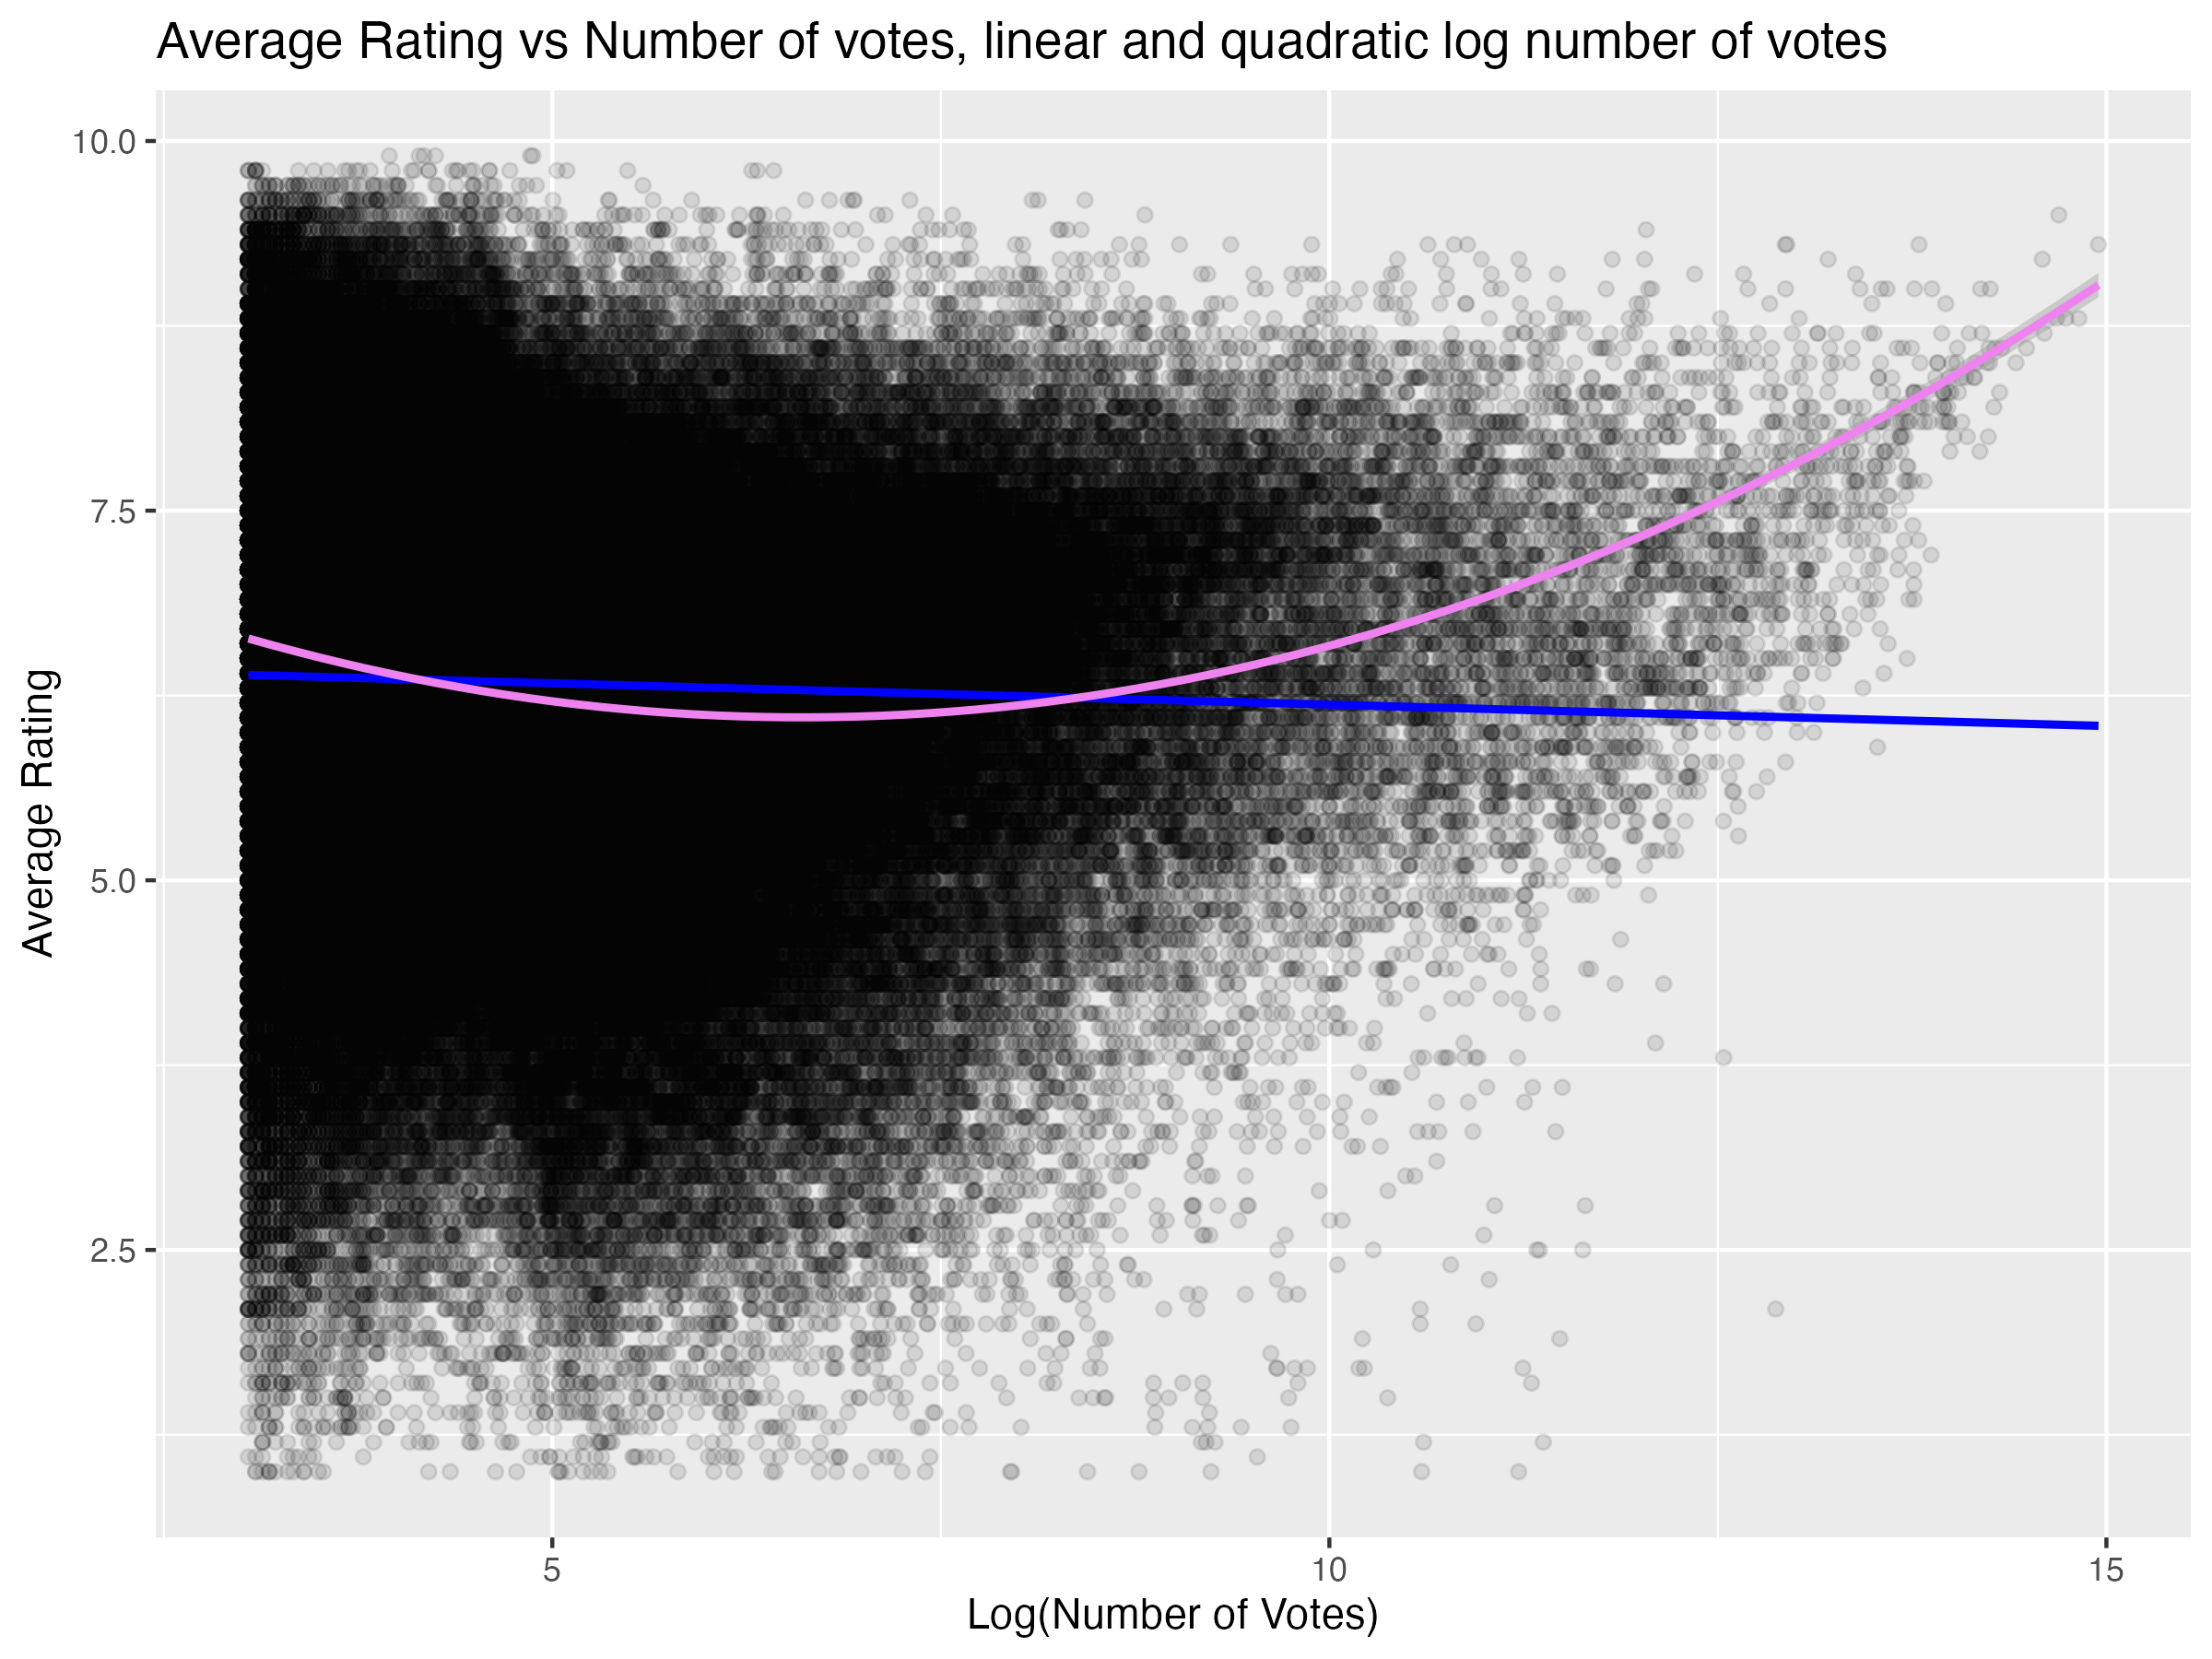
\includegraphics[keepaspectratio]{../../gen/output/model1_2.png}}
\caption{Average rating vs.~number of votes, linear and quadratic log
number of votes}
\end{figure}

\textbf{Model 3 -- Moderation by Genre Family.} The main effect of the
heavy genre is positive (β = +0.59, p \textless{} .001): heavy, serious
genres (drama, war, biography) tend to have higher ratings overall than
escapist genres (comedy, action). The interaction terms are small yet
significant: • log\_votes × genre\_familyHeavy: negative (β = --0.056, p
\textless{} .001) • log\_votes² × genre\_familyHeavy: positive (β =
+0.0049, p \textless{} .001) As such, the U-shaped curve is steeper for
heavy genres; i.e.~polarization is more pronounced for heavy titles.

\begin{figure}
\centering
\pandocbounded{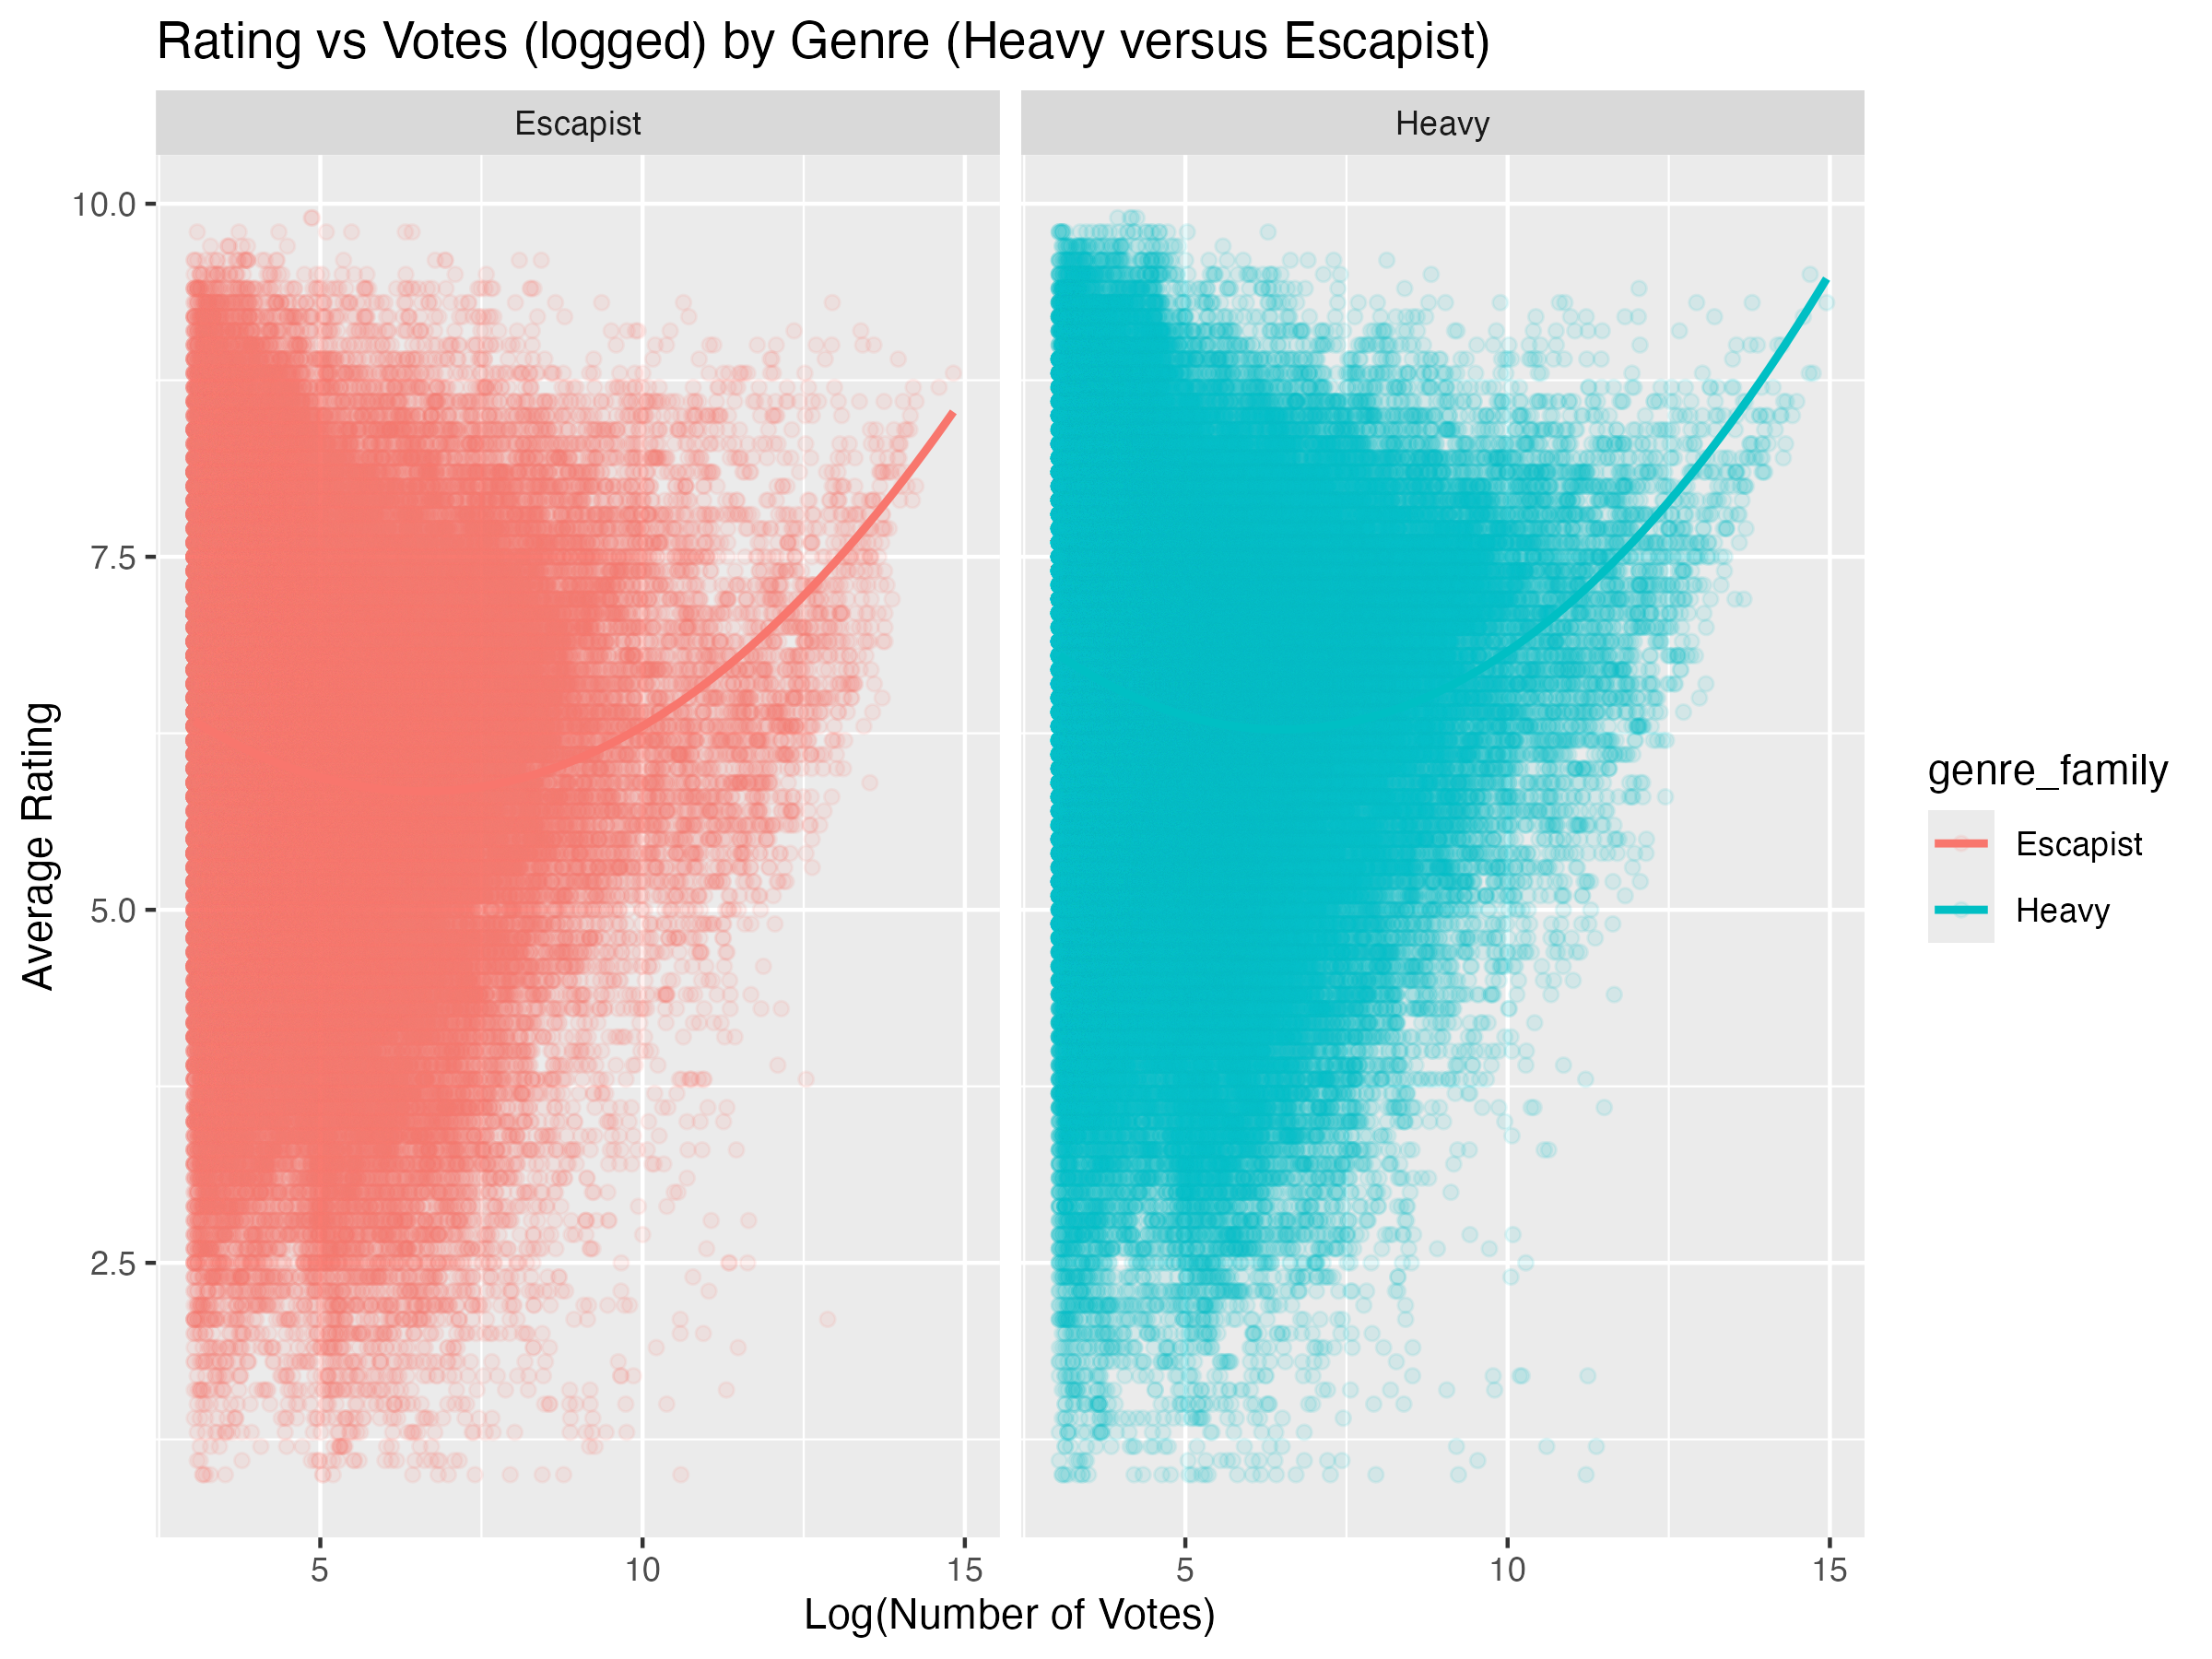
\includegraphics[keepaspectratio]{../../gen/output/model3.png}}
\caption{Rating vs.~Votes (logged) by Genre (Heavy vs.~Escapist)}
\end{figure}

\textbf{Model 4} -- Moderation by content type (movies vs.~series).
First, series are rated lower on average than movies (β = --0.26, p
\textless{} .001).The interaction pattern is opposite to the genre
effect: • log\_votes × series: positive (β = +0.299, p \textless{} .001)
• log\_votes² × series: negative (β = --0.0157, p \textless{} .001) The
main curve (for movies) is U-shaped, but for series, these interactions
flatten or even invert the curve.

\begin{figure}
\centering
\pandocbounded{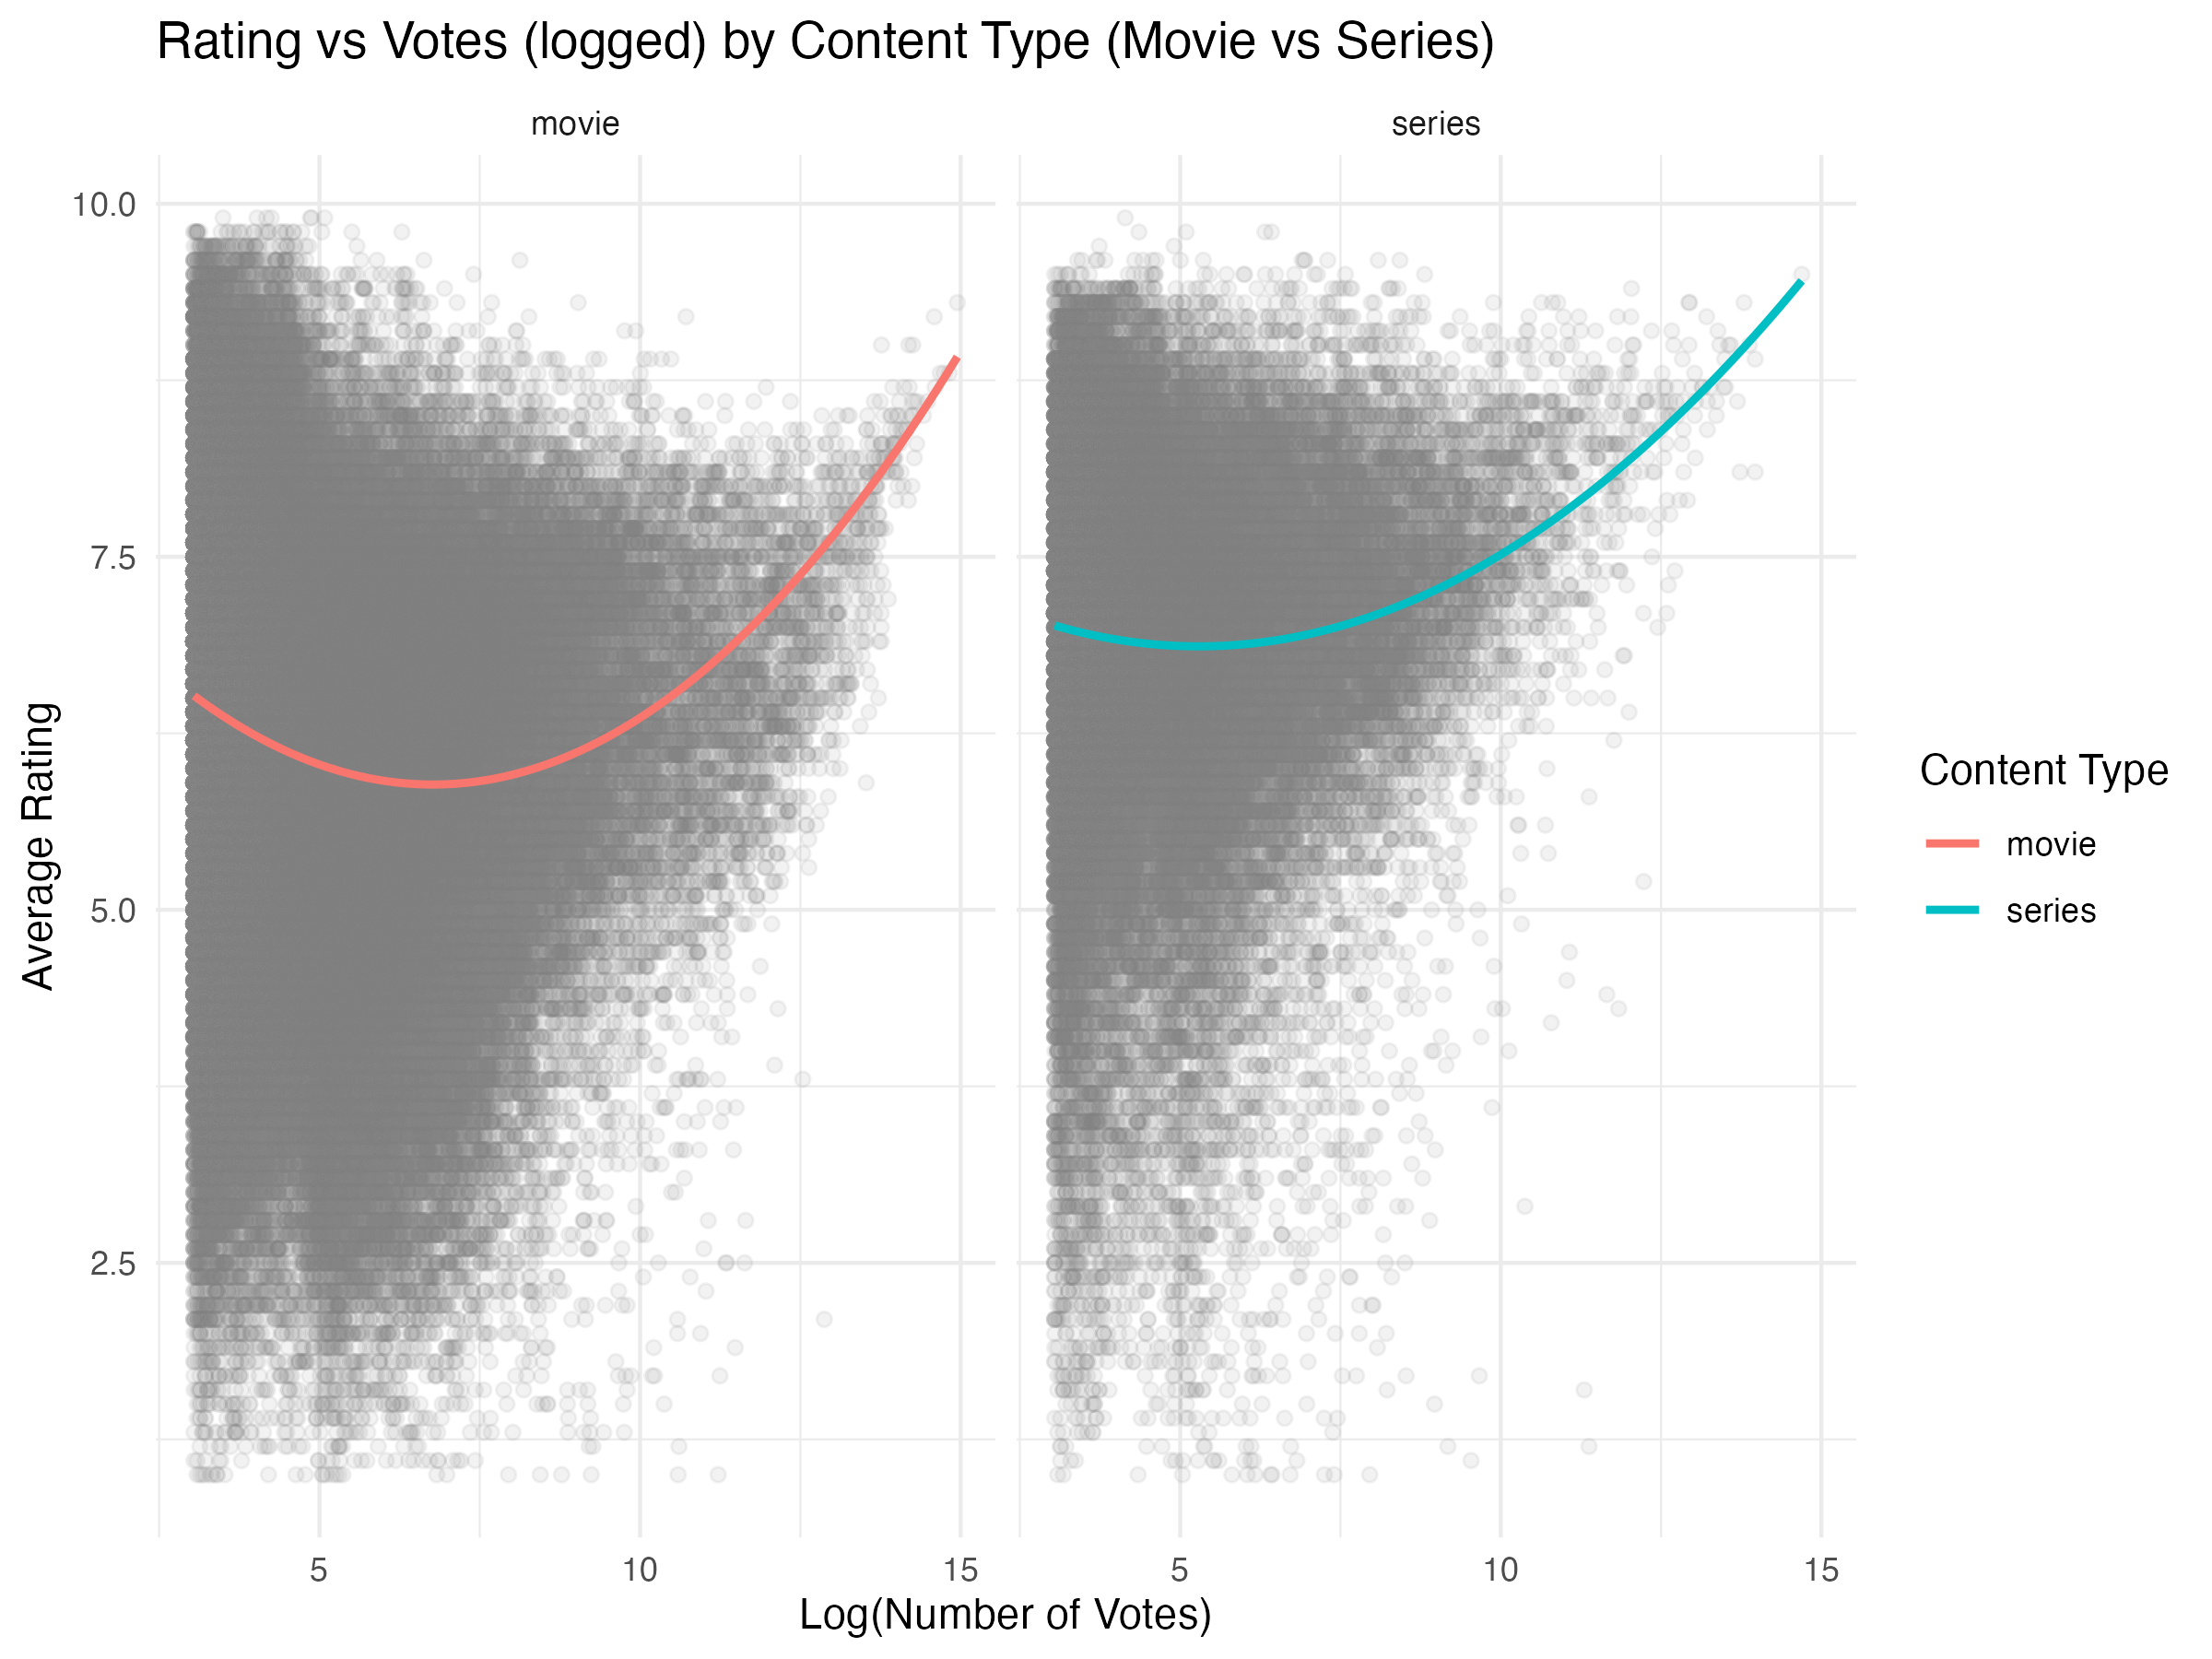
\includegraphics[keepaspectratio]{../../gen/output/model4.png}}
\caption{Rating vs.~Votes (logged) by content type (Movie vs.~Serie)}
\end{figure}

\#7. Conclusion and Recommendations The current study studied the the
relationship between the number of votes and the average rating of
movies on IMDb. Additionally, it explored whether this relationship
between number of votes and average rating differed across movie genres
(escapist (fantasy, comedy, romance) and heavy (drama, thriller)) and
across movies and series (i.e.~content form). Based on the results of
the study, we conclude that from a simple linear analysis it appears
that movies with more votes have a lower rating overall. However, adding
a quadratic term for number of votes, we conclude that titles with very
few or very many votes have higher ratings on average than those with a
moderately number of votes. --- either high praise or sharp criticism
--- while moderately popular titles receive more average evaluations.

Moreover, we conclude that audiences of heavy genres appear more
divided: some viewers rate these titles very highly, while others rate
them quite low. Escapist genres show a flatter relationship, suggesting
more uniform audience reception. Moreover, the type of content (movies
vs.~series) affects the relationship between number of votes and rating.
For movies, the polarization effect is evident: both very popular and
very niche films get stronger reactions.For series, however, the pattern
trends toward an inverted U-shape --- moderately popular series tend to
receive higher average ratings than very niche or extremely popular
ones.

Based on these findings, we offer several recommendations. First, for
platforms like IMDb, understanding the non-linear relationship between
the number of votes and average ratings can help in interpreting
consumer feedback more accurately. Moderately popular titles may appear
average not due to poor quality, but due to the tendency of extreme
ratings at the low and high ends to balance out.

Moreocer, content creators should consider the genre-specific
differences in audience reception. We note that genres are rated
differently: heavy genres (drama, thriller) tend to get more polarized
responses whereas escapist genres (fantasy, comedy, romance) generally
receive more uniform evaluations, indicating broader appeal. Marketing
strategies for heavy genres might thus target more specifically a niche
group of consumers who really like such content, boosting overall
ratings.

Third, the type of content influences audience reaction patterns. For
movies, extreme popularity or niche status often leads to stronger
audience reactions, while series tend to follow an inverted U-shape,
with moderately popular series receiving the highest ratings. This is
highly insightful for platforms such as Netflix or HBO for example,
which might prompt them to realize more satisfaction for average
mainstream series content, but more specific and niche video content.

\#8. Limitations and Future Research We note that our analysis is not
very granular and we do not control for differences between consumers.
This is partly due to unavailability of data on consumer characteristics
and also partly to limit the difficulty of the analysis and
interpretation. However, this is a great limitation to the extent that
differences between consumers may affect the study results, resulting in
erroneous conclusions. Future research should take into account more
controls, ensuring a limited influence of confounding factors.

Another limitation is the filtering of votes. As discussed we filtered
out titles with less than 20 votes, concluding that the ratings of less
than 20 consumers would not be representative for a general rating of a
title. However, the 20 votes cutoff is rather arbitrary; we could have
taken 40 or 50 as well or any other (low) number. By effect, we do
filter out some polarization as titles with fewer number of votes may be
rated more extreme. We realize this limitation but we also contend that
fewer votes (5 for example) may be arbitrary and do not represent
consumer opinions. Future research could explore whether other cutoffs
in number of votes would influence ratings.

Additionally, our study does not account for temporal effects. Ratings
may evolve over time as more consumers provide input. Ignoring these
dynamics may mask important patterns in the data and lead to conclusions
that do not generalize across time.

\section{Reproducibility \& Workflow}\label{reproducibility-workflow}

\begin{itemize}
\item
  The entire pipeline is automated via relative paths and can be run
  with a single make command from the repository root.
\item
  All raw data is downloaded programmatically; generated files are
  written to data/clean.
\item
  .gitignore excludes generated files to keep version control clean.
\item
  The repository follows the recommended directory structure
  (src/1-raw-data, data/clean, analysis).
\item
  Multiple team members contributed via commits, pull requests, and
  GitHub Issues/Project Board, ensuring transparency.
\end{itemize}

\section{Appendix}\label{appendix}

\begin{itemize}
\item
  Session info
\item
  Extra regression tables
\end{itemize}

\end{document}
